% PREAMBLE -- START

\documentclass[12pt,dvipsnames]{article}
\usepackage{amsmath,epsfig,subfigure,fancybox}
\usepackage{amsfonts,amssymb,amsthm,xparse}
\usepackage{rotating}
\usepackage{times}
\usepackage{bbm}
\usepackage{bm}
\usepackage{verbatim}
\usepackage{mathrsfs,wrapfig}
\usepackage{smartdiagram}
%\usepackage{physics}

\oddsidemargin .25in
\evensidemargin .25in  
\textwidth 6in
\topmargin -0.4in      
\textheight 8.75in

% New commands to make life easy

%
% short cuts
%

\newcommand{\eref}[1]{(\ref{#1})}
\newcommand{\fref}[1]{Fig.~\ref{#1}}
\newcommand{\tref}[1]{Table~\ref{#1}}
\newcommand{\sref}[1]{Section~\ref{#1}}
\newcommand{\vm}[1]{\mathbf{#1}}
\newcommand{\vx}{\vm{x}}
\newcommand{\bsym}[1]{\boldsymbol{#1}}
\newcommand{\abs}[1]{{\lvert#1\rvert}}
\newcommand{\norm}[1]{{\lVert#1\rVert}}
\newcommand{\inner}[2]{(#1,#2)}
\renewcommand{\mathbbm}[1]{\vm{#1}}

\newcommand{\incolor}[1]{\Red{#1}}

%\usepackage{hyperref}
\usepackage{url,color,colordvi}
\graphicspath{ {./figures/} }

% PREAMBLE -- END

\begin{document}

\title{Radial Density Functional Theory}
\author{Subhajit Banerjee and N. Sukumar}
\date{\today}
\maketitle

\begin{abstract}
The formulation and implementation of radial Density Functional 
Theory is presented.  
\end{abstract}

\section{Strong form}
Consider the case of an isolated atom. Let this atomic system consists of 
$N$ electrons. In an uncharged atom, the atomic number $Z$ is also 
equal to $N$. In the paradigm of many-b0dy quantum  
mechanics applied to such atomic systems one is interested determining the 
single-particle (electronic) \emph{wavefunctions} (\emph{orbitals}) $\{ \psi_i(x_i) \}$. 
For spherically symmetric potential, as is the case for an isolated atom, the 
wavefunctions are often expressed as $\psi_{n \ell m} (\vx)$ where $n$ is the principal quantum number, 
$\ell$ is the orbital angular momentum quantum number, and $m$ is the magnetic quantum number. 

\noindent
$\psi_{n \ell m} (\vx)$ can further be simplified (separation of variables):
$$\psi_{n \ell m} (\vx) \equiv \psi_{n \ell m} (r, \theta, \phi) = R_{n \ell}(r) Y_{\ell m}(\theta, \phi)$$
where $Y_{\ell m}(\theta, \phi)$ are the \emph{spherical harmonics} and $R_{n \ell}(r)$ satisfies the 
\emph{radial Schr{\"o}dinger equation}:
\begin{equation}	\label{radsch}
\Big( -\frac{1}{2} r^2 R^\prime_{n \ell}(r) \Big)^\prime + \Big( r^2 V(r) + \frac{1}{2} \ell (\ell + 1) \Big ) R_{n \ell}(r) = 
\varepsilon_{n \ell} r^2 R_{n \ell} (r)
\end{equation}
where $(\cdot)^\prime \equiv \dfrac{d(\cdot)}{dr}$.
\noindent
In \emph{Radial Density Functional Theory} the \emph {radial Kohn-Sham equation} is solved in a \emph{self consistent} manner. 
The radial Kohn-Sham equation, in spirit, is of similar form as eq.~\eqref{radsch} with the potential $V(r)$ 
being replaced by $\hat{V}_{\rm{eff}}[\rho_e(r)]$ where $\rho_e$ is the \emph{electronic density}. 
Hence, eq.~\eqref{radsch} can be rewritten as:
\begin{equation}	\label{radks}
\Big( -\frac{1}{2} r^2 R^\prime_{n \ell}(r) \Big)^\prime + \Big( r^2 \hat{V}_{\rm{eff}}[\rho_e(r)] + \frac{1}{2} \ell (\ell + 1) \Big ) R_{n \ell}(r) = 
\varepsilon_{n \ell} r^2 R_{n \ell}(r)
\end{equation}
where 
\begin{equation} \label{veff}
\hat{V}_{\rm{eff}}[\rho_e(r)] = V_H[\rho_e(r)] + V_{xc}[\rho_e(r)] + V_n(r).
\end{equation}
In eq.~\eqref{veff} $V_{xc}$ is known as the \emph{exchange-correlation} functional, 
$V_n(r) = -\frac{Z}{r}$ is the potential arising from the coulomb attraction of nucleus and $V_H$ is 
the \emph{Hartree potential}. The Hartree potential is governed by the \emph{radial Poisson 
equation}:
\begin{equation} \label{radpois}
\frac{1}{r^2} \Big( r^2 V^\prime_H(r) \Big)^\prime = V^{\prime \prime}_H (r) + \frac{2}{r} V^\prime_H(r) = -4 \pi \rho_e(r).
\end{equation}

\noindent
Note that eq.~\eqref{radks} is a nonlinear ordinary differential equation. This can further be 
elucidated by expressing $\rho_e(r)$ in terms of $R_{n \ell}$ which is done next. 
%
\subsection{Electron Density $\rho_e$} \label{sec:nonlin}
The electronic density $\rho_e$ is calculated by adding all $(n, \ell, m)$ states together, counting each one
twice (for spin up $\uparrow$ and spin down $\downarrow$) such that
\begin{align*}
\rho_e(r) & = 2 \sum\limits_{n \ell m} \vert \psi_{n \ell m} \vert^2 \\
& = 2 \sum\limits_{n \ell m}  R_{n \ell}^2 \vert Y_{\ell m} \vert^2\\
& = \Big( \sum\limits_{n \ell} R_{n \ell}^2 \Big) \Big(2 \sum\limits_m \vert Y_{\ell m} \vert^2 \Big) =  \frac{1}{4 \pi} \sum\limits_{n \ell} f_{n \ell} R_{n \ell}^2
\end{align*}
where the \emph{occupation numbers} $f_{n \ell}$ are defined as
\begin{equation}		\nonumber
f_{n \ell} = 2 \Big( 4 \pi \sum\limits_m \vert Y_{\ell m} \vert^2 \Big).
\end{equation}
Hence, we get the following circular dependency:\\
\begin{center}
\smartdiagram[flow diagram:horizontal]{$\rho_e$, $\hat{V}_{\rm{eff}}$, $R_{n \ell}$}
%\smartdiagram[circular diagram:clockwise]{$\rho_e$, $\hat{V}_{\rm{eff}}$, $R_{n \ell}$}
\end{center}
%
\subsection{$P_{n \ell}$ and $V_P$}
Please note that in the code \texttt{spectatom} we use $u = P_{n \ell} = r R_{n \ell}$
and $V_P = r V_H$ as our primary variables to be solved using spectral FEM. 
This is solely because of some obvious simplification in the boundary conditions. 
To this end, the aforementioned strong form statements are modified for these variables 
as:\\

\noindent
{\bf Radial Kohn-Sham Equation:}
\begin{equation}
-\frac{1}{2} \big( P_{n \ell}[\rho_e(r)] \big)^{\prime\prime} + \Big(r^2 \hat{V}_{\rm{eff}}[\rho_e(r)] + \frac{1}{2} \ell (\ell + 1) \Big) P_{n \ell}[\rho_e(r)] = \varepsilon_{n \ell}[\rho_e(r)] P_{n \ell}[\rho_e(r)];
\end{equation}

\noindent
{\bf Radial Poisson Equation:}
\begin{equation}
\big(V_P(r)\big)^{\prime\prime} = -4 \pi r \rho_e(r),
\end{equation} 
and lastly\\
{\bf Electron Density:}
\begin{equation}
\rho_e(r) = \frac{1}{4 \pi} \sum\limits_{n \ell} f_{n \ell} \frac{R_{n \ell}^2}{r^2}.
\end{equation}
%
%
\section{Weak form}
The weak form statements of the radial Kohn-Sham problem ($P_{n \ell}$ as the 
primary variable) and radial Poisson problem ($V_P$ as the primary variable) are stated next 
without any derivation. To this end, we first define the following function spaces:
\begin{align*}
{\cal S} &= \{ P: P \in H^1([0 \, \, a]), \ P(0) = 0, \ P(a) = 0 \}, \\
{\cal V} &= \{ v: v \in H^1([0 \, \, a]), \ v(0) = 0, \ v(a) = 0 \},
\end{align*}
where $a$ denotes the radius of the spherical problem domain under consideration, 
$H^k([0 \, \, a])$ is the \emph{Sobolev space} that contains
functions that are square-integrable ($L^2([0 \, \, a])$) up to order $k$.
%
\subsection{Radial Kohn-Sham Equation}
Formally, the weak form is written as: find the \emph{trial function} (eigenfunction) 
$P_{n \ell}(r) \in {\cal S}$ and the eigenvalue $\varepsilon_{n \ell} \in \mathbb{R}$
such that
\begin{multline} \label{weakksP}
\int\limits_{0}^a \Big\{ \frac{1}{2} P^\prime_{n \ell}(r) v^\prime(r) + \Big [ \hat{V}_{\rm{eff}}[\rho_e(r)] + \frac{1}{2}\frac{\ell(\ell + 1)}{r^2} \Big ]
P_{n \ell}(r) v(r) \Big\} \, \mathrm{d} r  = \\
\varepsilon_{n \ell} \int\limits_{0}^a P_{n \ell} (r) v(r) \, \mathrm{d} r \qquad \forall v(r) \in {\cal V}.
\end{multline}
Observe that we use  $P_{n \ell}(0) = P_{n \ell}(a) = 0$, i.e., 
Dirichlet condition at both ends.
%
\subsection{Radial Poisson Equation}
The weak form statement of radial Poisson equation is: 
find the trial function $V_P(r) \in {\cal S}$ such that
\begin{equation} \label{weakpoisVp}
\int\limits_{0}^a V^\prime_P(r) w^\prime(r) \, \mathrm{d} r = 4 \pi \int\limits_{0}^a r \rho_e(r) w(r) \, \mathrm{d} r \qquad \forall w(r) \in {\cal V}
\end{equation}
where the trial and test function spaces are as defined previously. Note here that we 
use $V_P(0) = V_P(a) = 0$ as the boundary condition and this defines $V_H = \frac{V_P}{r}$ 
within some arbitrary constant. Physically, $V_H(a) = \frac{Z}{a}$ should be satisfied. 
Hence, we first compute $V_P$ using eq.~\eqref{weakpoisVp} and then scale and shift the solution 
as 
\begin{equation*}
V_H = \underbrace{\frac{V_P}{r}}_{\textrm{Scale}} + \underbrace{\frac{Z}{a}}_{\textrm{Shift}}
\end{equation*}
to obtain $V_H(r)$.
%
\section{Discrete Formulation of Weak Form}
\subsection{Radial Kohn-Sham Equation}
The spectral finite element (FE) approximation of the trial function $P_{n \ell}$ 
can be written as (dropping the subscripts $n$ and $\ell$ for brevity)
\begin{equation}	\label{eq:fem}
P^h (r) = \sum_{j=1}^N \phi_j(r) P_j \in {\cal S}^h \subset {\cal S},
\end{equation}
where ${\cal S}^h$ is a finite-dimensional subspace of ${\cal S}$. In
addition, $\phi_j(r)$ are higher-order (spectral) finite element 
basis functions, and $P_j$ are the finite element degrees of freedom. 
The derivative of $P^h(r)$ is:
\begin{equation}\label{eq:dfem}
\bigl(P^h(r)\bigr)^\prime = \sum_{j=1}^N \phi_j^\prime (r) P_j.
\end{equation}

\noindent
On substituting $P^h$ and $(P^h)^\prime$ from~\eref{eq:fem} and~\eref{eq:dfem}, respectively, in eq.~\eqref{weakksP}
 and letting $v^h$ be the test functions, we obtain:
\begin{multline*}
\int_0^a \Big\{ \sum_{j=1}^N \Big( \frac{1}{2} (v^h)^\prime \phi_j^\prime + 
\Big[ \hat{V}_{\rm{eff}} + \frac{1}{2}\frac{\ell(\ell + 1)}{r^2} \Big ] v^h \phi_j \Big ) P_j \Big\} \mathrm{d} r = \\
\varepsilon \int_0^a \sum_{j=1}^N v^h \phi_j P_j \mathrm{d} r \qquad \forall v^h \in {\cal V}^h.
\end{multline*}
Upon setting $v^h = \phi_i$ and denoting by $\vm{c} = \{P_1, \ldots, P_N\}$ leads to the \emph{ generalized eigenproblem}:
\begin{subequations}\label{eq:eigproblem}
\begin{align}
\vm{H} [\rho_e(r)] \vm{c} &= \varepsilon \vm{S} \vm{c}, \label{geneig}\\
\big(\vm{H}[\rho_e(r)]\big)_{ij} & = \int_0^a \Big\{ \frac{1}{2} \phi_i^\prime \phi_j^\prime + 
\Big[ \hat{V}_{\rm{eff}} + \frac{1}{2} \frac{\ell(\ell + 1)}{2 r^2} \Big ] \phi_i \phi_j \Big\} \mathrm{d} r \\
\vm{S}_{ij} & =  \int_0^a \phi_i \phi_j \mathrm{d} r.
\end{align}
\end{subequations} 
In the context of Schr\"odinger equation, $\vm{H}[\rho_e(r)]$ is known as the \emph{Hamiltonian matrix} and 
$\vm{S}$ is the \emph{overlap matrix}.
%
\subsection{Radial Poisson Equation}
Proceeding along the similar line as in the last section, the spectral finite element 
approximation for the trial function $V_P$ can be written as (dropping the subscript $P$ for brevity)
\begin{equation}	\label{eq:femV}
V^h (r) = \sum_{j=1}^N \phi_j(r) V_j \in {\cal S}^h \subset {\cal S}.
\end{equation}
In addition, $\phi_j(r)$ are higher-order (spectral) finite element 
basis functions, and $V_j$ are the finite element degrees of freedom. 
The derivative of $V^h(r)$ is:
\begin{equation}\label{eq:dfemV}
\bigl(V^h(r)\bigr)^\prime = \sum_{j=1}^N \phi_j^\prime (r) V_j.
\end{equation}
On substituting $V^h$ and $(V^h)^\prime$ from~\eref{eq:femV} and~\eref{eq:dfemV}, 
respectively, in eq.~\eqref{weakpoisVp} and letting $w^h$ be the test functions, we obtain:
\begin{equation*}
\int_0^a \Big\{ \sum_{j=1}^N (w^h)^\prime \phi_j^\prime V_j \Big\} \mathrm{d} r = 4 \pi \int_0^a r \rho_e w^h \mathrm{d} r \qquad \forall w^h \in {\cal V}^h.
\end{equation*}
Once again, setting $w^h = \phi_i$ and denoting by $\vm{u} = \{V_1, \ldots, V_N\}$ leads to the linear system:
\begin{subequations}\label{eq:linsys}
\begin{align}
\vm{K}\vm{u} &= \vm{b}, \\
\vm{K}_{ij} & = \int_0^a \phi_i^\prime \phi_j^\prime \mathrm{d} r \\
\vm{b}_i & = 4 \pi \int_0^a r \rho_e \phi_i \mathrm{d} r.
\end{align}
\end{subequations}
%
\newpage
\section{Self-Consistent Fields (SCF) Iterations}
Owing to the nonlinear nature of generalized eigenvalue problem in eq.~\eqref{geneig} as 
alluded in Section~\ref{sec:nonlin}, the problem is solved using the following self-consistent 
field technique:
\begin{center}
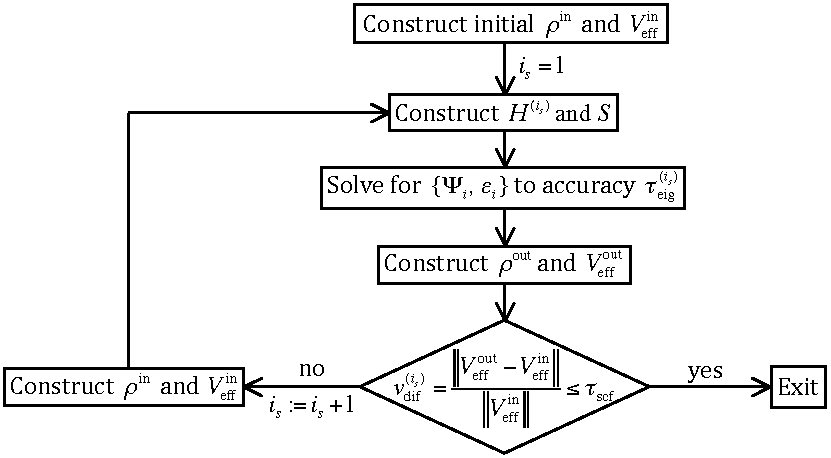
\includegraphics[width=1\textwidth]{scf.pdf}
\end{center}
%
%
\section{Numerical Examples}
We perform $h$- and $p$- convergence studies on ground state energy ($E_0$) computation for 
carbon (C) atom which has $6$ electrons. As per the {\bf NIST} standard the $E_0$ for C is $(E_0)_{\textrm{exact}} = -37.425749$ Hartree. 
To this end, we consider the domain $[\texttt{rmin} \, \, \texttt{rmax}] = [0 \, \, 10]$ a.u., meshed with \texttt{numel} equi-spaced 
elements.
%
\subsection{$p$-Convergence} 
For a fixed \texttt{numel} the element order $p$ is varied as $1, 2, \ldots, 10$ . For each of these $p$, $E_0$ value is 
reported. Increasing $p$ increases the number of DOF and hence, ideally we should converge to the $(E_0)_{\textrm{exact}}$. 
Subsequently, we also consider $\texttt{numel} = 10, 20$, and $40$. This set of numerical experiments are performed using 
the script \texttt{testpconvergence.m}.
%
\begin{figure}[h!]
	\centering
	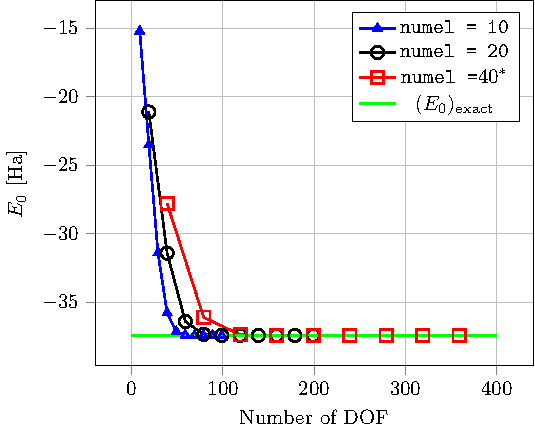
\includegraphics[width=1\textwidth]{pconv.pdf}
	\caption{p-Convergence ($\ast$ \texttt{eigs} failed for $\texttt{numel} = 40$ with $p = 10$)}
\end{figure}
%
\subsection{$h$-Convergence}
For a fixed element order $p$ the element order \texttt{numel} is varied as $5, 10, 20,$ and $40$. 
For each of these \texttt{numel}, $E_0$ value is reported. Increasing \texttt{numel} once again increases the 
number of DOF and hence, ideally we should converge to the $(E_0)_{\textrm{exact}}$. 
Cases with $p = 2, 4$, and $8$ are considered. This set of numerical experiments are performed using  
the script \texttt{testhconvergence.m}.
\begin{figure}[h!]
	\centering
	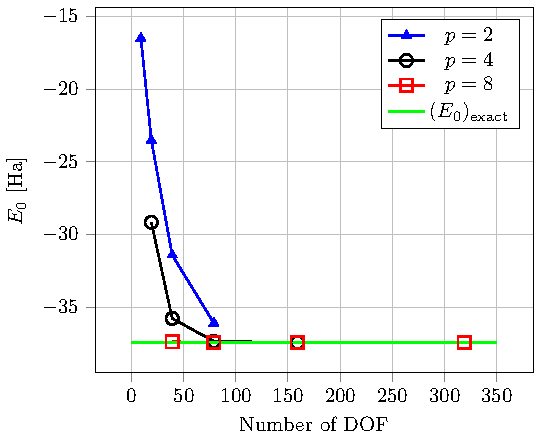
\includegraphics[width=1\textwidth]{hconv.pdf}
	\caption{h-Convergence}
\end{figure}











\end{document}
